\documentclass[12pt]{article}

\usepackage[margin=1in]{geometry}
\usepackage{mathptmx}
\usepackage{setspace}
\doublespacing
\usepackage{ragged2e}
\RaggedRight
\usepackage{microtype}
\usepackage{booktabs}
\usepackage{tabularx}
\usepackage{longtable}
\usepackage{array}
\usepackage{graphicx}
\usepackage{amsmath}
\usepackage{enumitem}
\usepackage{xurl}
\usepackage[hidelinks]{hyperref}
\usepackage[numbers,square,sort&compress]{natbib}

\setlength{\parindent}{0.5in}
\setlength{\parskip}{0pt}
\setlength{\emergencystretch}{2em}
\setcounter{secnumdepth}{3}
\setcounter{tocdepth}{2}
\pagestyle{plain}

\newcommand{\placement}[1]{%
  \begin{center}
    \vspace{0.5\baselineskip}
    \textit{[Insert #1 about here]}
    \vspace{0.5\baselineskip}
  \end{center}
}

\title{Beyond AI Mentions: Attention Growth and Operational Artificial
Intelligence Disclosure in Corporate Filings}
\author{}
\date{}

\begin{document}

\maketitle
\thispagestyle{plain}


\begin{abstract}
Corporate AI references do not establish operational use. This study separates
AI attention from disclosures of current or completed deployment in U.S. SEC
filings from 2017 to 2025. A frozen open-weight language model classifies
26,279 lexicon-positive passages; a probability audit of 1,000 reference-coded
passages corrects classification error. The original 200-passage reference
set was human coded and then AI-assisted in adjudication; assistance during
correction of the additional 800 is not documented. From 2017--2022 to 2023--2025,
AI-related passages per 100 filings increased 6.3-fold, whereas
human-corrected operational passages increased 3.3-fold. Consequently, the
operational share fell from 25.76\% to 13.45\%; a sector-and-form decomposition
shows that the decline persists within comparable reporting contexts, while
the composition component is small and imprecise. Overall corrected
prevalence is 16.53\% (approximate 95\% Wald interval: 14.03\%--19.03\%).
The results show that rapidly expanding organizational communication about AI
can outpace growth in disclosed operational use.
\end{abstract}


\noindent\textbf{Keywords:} artificial intelligence adoption; corporate
disclosure; large language models; prediction-powered inference; SEC filings;
organizational technology use

\section{Introduction}

Artificial intelligence has become an organizational technology whose
operational use is difficult to observe consistently. Firms can discuss AI
without deploying it, and they can deploy it without disclosing the activity.
Patents, AI-skilled employees, surveys, websites, and regulatory text therefore
capture related but distinct objects: invention, capability, reported use,
planned adoption, and communication. Interpreting these indicators as
interchangeable can obscure the organizational state that an empirical
measure actually represents.

This study addresses a specific question: when corporate discussion of AI
expands, how much of that growth represents disclosed operational use?
Operational AI-use disclosure is defined as a statement that identifies the
organizational actor, the technology, the activity to which it is applied, and
evidence of current use or completed implementation. Plans, pilots, generic
discussion, and insufficiently specified claims are distinguished from
operational use. The target is a public claim about deployment, rather than
verified real-world adoption.

The empirical setting comprises 26,279 lexicon-positive passages from SEC
filings associated with historical S\&P 500 membership during 2017--2025.
A frozen language-model system classifies the candidate corpus. Human labels
for a probability-sampled audit of 1,000 passages then correct aggregate
human--model discrepancies through prediction-powered inference. Machine
predictions provide coverage; human reference judgments and their sampling
design determine the correction and its uncertainty.

The principal finding is a divergence between communication volume and
operational content. Comparing 2017--2022 with 2023--2025, retained
AI-related passages rose from 29.31 to 185.38 per 100 eligible filings, a
6.3-fold increase. Human-corrected operational passages rose from 7.55 to
24.94 per 100 filings, a 3.3-fold increase. The operational share of candidate
passages consequently fell from 25.76\% to 13.45\%, a decline of 12.31
percentage points, or 47.8\%. Conditioning jointly on sector and filing form
produces a within-context decline of 13.39 percentage points; the estimated
composition component is small and imprecise.

Across all years, human-corrected prevalence is 16.53\%, compared with a raw
model-positive rate of 11.60\%. The approximate design-based 95\% interval is
14.03\%--19.03\%. Weighted precision of 80.6\% accompanies recall of 56.6\%
and specificity of 97.3\%. These findings illustrate why rapid growth in AI
language, high specificity, and a plausible raw count are each insufficient
to establish growth in operational content.

The paper connects a bounded operational-disclosure construct to a
theory-informed distinction between organizational communication and
operational content. Institutional legitimacy and symbolic-management
arguments motivate competing expectations about the operational share of
AI-related disclosure. A benchmark and decomposition framework distinguishes
expansion in attention, changes within organizational contexts, and changes
in the composition of disclosing contexts.
The statistical correction builds on established prediction-powered inference;
its application is not presented as a new estimator. A further design
implication is that stratification on the model prediction can make aggregate
PPI algebraically equivalent to direct design-weighted human estimation.
The organizational contribution therefore depends on the content and
heterogeneity of disclosure, rather than an assumed extra precision gain.

\placement{Table 1}

\section{Literature Review and Research Positioning}
\label{sec:literature}

Artificial intelligence is increasingly treated as an organizational
technology, yet its use remains difficult to observe. Existing studies address
this problem through proxies that capture different parts of the adoption
process. Patents identify inventive activity and accumulated technical
knowledge \citep{igna2023innovation}; employee resumes capture investment
in AI-related human capital \citep{babina2024growth}; and business surveys
ask firms whether they use particular AI technologies
\citep{mcelheran2024adoption}. More recently, researchers have used
transformer models to identify AI activity from firm websites and trace its
diffusion across industrial and regional networks
\citep{dahlke2024epidemic}. This work demonstrates that AI adoption is
uneven and depends on complementary organizational resources. It also reveals
a measurement problem. Patenting, hiring, experimenting with, and deploying AI
are not equivalent activities. A measure that is informative about one stage
cannot automatically be interpreted as evidence of another.

Corporate disclosures offer a different view of this process. Unlike patents
or labor-market records, regulatory filings contain firms' own descriptions of
their technologies, business processes, risks, and expected effects. They can
therefore reveal where managers locate AI within the organization and how they
present its role to investors. At the same time, disclosure is not a neutral
record of organizational reality. Firms decide what is material, how
specifically to describe it, and whether to emphasize opportunities or risks.
Evidence from cybersecurity disclosure shows that these choices respond to
public and institutional pressures \citep{darcy2022disclosures}; firms also
adjust disclosure language when they expect machines to read their reports
\citep{cao2023machine}. SEC filings should consequently be understood as a
selective observation of organizational activity, not as a complete inventory
of it.

Recent studies show why this distinction is especially important for AI.
\citet{anantharaman2026disclosure} document a sharp increase in AI-related
10-K disclosure after the release of ChatGPT and connect that disclosure to
firms' AI exposure and capital-market information outcomes. Evidence from
conference calls likewise shows that managers increasingly discuss
generative-AI initiatives \citep{jia2026genai}, while research on
AI-adoption announcements finds that market reactions depend on the
combination of substantive capability claims and rhetorical signals
\citep{nishant2024signals}. These studies establish that AI communication
contains meaningful information. However, they also leave unresolved what an
AI mention represents. The same term can appear in a description of current
internal use, a future plan, an experimental pilot, a product sold to
customers, a hypothetical threat, or a general discussion of industry change.
Counting these passages together conflates materially different organizational
states.

This problem is addressed through the construct of \emph{operational AI-use
disclosure}. It refers specifically to a passage in which a firm reports that
AI is currently used, or has completed implementation, in a business function.
The construct is narrower than corporate AI disclosure, which includes any
discussion of AI, and more observable than actual organizational AI use, which
may remain undisclosed. This positioning imposes an important claim boundary:
the study measures disclosed operational use, not the full universe of AI
deployment. A positive passage provides evidence of a firm's public claim;
absence of such a passage does not establish nonadoption. The distinction also
corresponds to the SEC Investor Advisory Committee's recommendation that firms
define AI and separately describe material deployment in internal operations
and consumer-facing activities \citep{sec2025recommendation}.

Identifying operational-use claims at scale requires semantic classification,
because the distinction depends on context rather than the presence of a
keyword. Large language models are well suited to this task, and recent
research reports strong performance in text annotation
\citep{gilardi2023annotation,mellon2024open}. Yet performance varies across
constructs and tasks \citep{ziems2024css}. Model outputs must therefore be
treated as fallible measurements rather than observed facts. This is not
resolved by reporting accuracy alone: asymmetric false positives and false
negatives can bias a population prevalence even when overall predictive
performance appears strong.

Prior IS research already recognizes that machine-generated variables can
transmit measurement error into subsequent analysis. Qiao and Huang
\citep{qiao2025measurement} examine correction of errors in aggregated
classification outputs used in regression models. Mousavi et al.
\citep{mousavi2026psychometric} compare approaches to psychometric text
measurement and examine annotation quality. The present study addresses a
different construct and inferential target: operational-use claims in corporate
disclosures and their finite-population passage prevalence. Applying established
prediction-powered inference is not itself presented as a new statistical
estimator; the proposed contribution lies in the construct specification,
traceable disclosure classification, and evaluation of aggregate measurement
error in a defined corporate-text population.

The resulting gap lies at the intersection of organizational AI research,
corporate disclosure, and machine-assisted measurement. Existing work provides
important evidence on AI investment and adoption, the content and consequences
of AI communication, and the use of language models as classifiers. The present study focuses on the narrower task of estimating operational
AI-use disclosure prevalence within a defined regulatory-text candidate frame
while accounting for machine classification error. A prespecified language model is combined
with a probability sample of 1,000 subsequently collected human labels, and
prediction-powered inference is used to correct the census predictions
\citep{angelopoulos2023ppi}. This design allows automated classification to
provide scale while human judgments determine the correction. The contribution
is therefore not another count of AI mentions, nor a claim to observe all
organizational AI use. It is a measure of the share of candidate passages that disclose operational
use, accompanied by an explicit distinction between that passage-level estimand
and firm-level adoption.

Building on this gap, the empirical analysis is organized around three tasks:
constructing the universe of AI-related passages, distinguishing operational
use from other AI references, and correcting aggregate estimates for
classification error. The following section describes the filing corpus,
measurement procedure, human-validation design, and statistical estimator.

\section{Theoretical Framing and Empirical Expectations}

\subsection{Institutional attention and operational content}

Institutional theory separates conformity to recognized organizational forms
from the activities through which work is performed. Meyer and Rowan
\citep{meyer1977institutionalized} explain why legitimacy-seeking structures
can become decoupled from technical activities. Fiss and Zajac
\citep{fiss2006symbolic} examine how firms frame strategic change and how
espousal can differ from implementation. Applied to AI disclosure, these
arguments suggest a reason to distinguish discussing a salient technology
from making a specific claim about its current organizational use. This is
an application of the theoretical lens, rather than evidence that a firm is
misrepresenting its activity.

An increase in AI-related communication can arise through at least two
processes. External attention can encourage discussion of opportunities,
risks, and intentions before operational implementation is disclosed.
Alternatively, complementary capabilities and organizational learning can
produce more operational content within that discussion. Both processes can
increase the volume of AI language; they imply different changes in the
operational share of that language. Public text can discriminate between
these disclosure patterns without directly identifying managers' motives or
verifying underlying deployment.

\textit{Expectation 1a (attention expansion with dilution).} If growth in
AI-related communication outpaces growth in operational-use claims, the share
of candidate passages meeting the operational criterion decreases in the
later period, even when keyword-positive disclosure intensity increases.

\textit{Expectation 1b (operational-content deepening).} If operational-use
claims grow faster than other AI-related communication, the operational
share increases in the later period. Persistence of that increase after
holding sector and filing-form composition fixed is consistent with change
within organizational reporting contexts.

These expectations are competing interpretations of a two-sided period
contrast. They are not both treated as supported by any nonzero result, and a
wide interval or a near-zero contrast leaves the comparison unresolved. The
2017--2022 versus 2023--2025 split summarizes periods around increased
AI salience; it is not a causal design for the release of ChatGPT.

\subsection{Organizational context and compositional change}

Organizational capabilities and disclosure incentives vary across business
contexts. AI-skilled labor and complementary resources differ across firms
\citep{babina2024growth,mcelheran2024adoption}, while stakeholder audiences
can influence how organizational change is framed \citep{fiss2006symbolic}.
An aggregate trend can consequently reflect a shift toward sectors or filing
types with higher operational disclosure, even when the operational share
within each context is unchanged or declining.

\textit{Expectation 2 (heterogeneous disclosure change).} The period change
in the operational share differs across sectors. A sector-by-period contrast
examines this expectation, while standardization separates changes within
sector or sector--form contexts from changes in their representation in the
candidate corpus. This is a descriptive interaction, not causal
difference-in-differences.

The relevant organizational question is therefore whether growth in AI
communication contains more operational content within comparable contexts,
or instead reflects a different mix of organizations and documents. A
comparison of keyword-positive and operational disclosure intensities also
shows whether a mention-based ordering of sectors survives semantic
classification and human correction. Table~\ref{tab:expectations} maps the
mechanisms to observable contrasts. These extensions were developed after
the aggregate results were known and are identified as exploratory rather
than preregistered hypotheses.

\placement{Table 2}

\section{Data and Methodology}
\label{sec:methodology}

\subsection{Data}

The empirical setting consists of firms included in the S\&P 500 at some
point between January 1, 2017, and December 31, 2025. Historical index
membership was used to determine eligibility during this period rather than
applying the constituent list from a single date. The resulting universe
contains 684 firms, of which 653 had at least one eligible filing. Firms were
linked across filings through their SEC Central Index Key (CIK). Available
GICS sector classifications are used for descriptive comparisons; these
fields reflect static metadata and are not interpreted as historical
point-in-time sector assignments.

The documents were obtained from the U.S. Securities and Exchange Commission
(SEC) EDGAR database. The corpus includes Forms 10-K, 10-Q, Form 8-K
Item 2.02 earnings releases, and eligible earnings exhibits. These filing
types provide annual, interim, and event-driven accounts of firms'
technologies, products, business processes, and risks. Filing year is defined
as the calendar year of the SEC filing date.

The initial frame contained 33,077 eligible SEC accessions. Of these, 33,064
were successfully processed; 13 records were unavailable in the processed
source collection. The final filing corpus contains approximately 22.9
million usable sentences, including filings in which no AI-related passage was
identified.

The processed exposure frame contains 4,175 Form 10-K, 12,648 Form 10-Q, and
16,241 eligible Form 8-K accessions. Retained candidates occur in 1,630 10-Ks,
1,986 10-Qs, and 499 8-Ks, yielding 14,639, 10,672, and 968 candidate
passages, respectively. Thus only 3.07\% of processed eligible 8-K accessions
contain a retained candidate, compared with 39.04\% of 10-Ks and 15.70\% of
10-Qs. This audit establishes the realized corpus coverage; it does not prove
complete retrieval of every potentially eligible EDGAR exhibit. Because the
8-K candidate yield is low and declines sharply after 2022, the temporal
analysis includes an explicitly post hoc 10-K-only robustness check.

Document formatting, tables, navigation material, and other nonnarrative
elements were removed before sentence segmentation. Character offsets and
source identifiers were preserved throughout processing. Each classification
passage consists of a target sentence together with its immediately preceding
and following sentences, when available. Individual passages are classified
for operational AI use, and the primary estimate measures the prevalence of
such disclosures across the candidate-passage corpus.

Each passage is linked to its CIK, SEC accession number, filing date, filing
form, source location, and text offsets. These links preserve sufficient
context for classification and allow each observation to be traced to its
source filing. The unit of analysis is the candidate passage; source links preserve the
distinction between text classification and firm-level aggregation.
Eight candidate-free filing-frame records carried legacy labels
``Telecommunication Services'' or ``Telecommunications Services.'' These
labels are harmonized to the current ``Communication Services'' category
before sector exposure is calculated. Passage metadata and all other sector
labels are left unchanged. Sector fields remain static descriptive metadata,
not point-in-time GICS classifications.

To improve computational efficiency, a deterministic prefilter was applied
before language-model classification. The prefilter uses a predefined list of
48 AI-related terms and their normalized spelling and hyphenation variants.
The list includes general expressions, such as ``artificial intelligence''
and ``machine learning,'' as well as terms referring to specific AI
technologies and applications. A passage entered the candidate set whenever
its normalized text contained at least one listed term. No semantic score or
estimated relevance threshold was applied at this stage.

The prefilter identified 26,420 raw candidate passages. The 100 passages used
for development and their associated context windows were excluded, removing
141 records and leaving $N=26{,}279$ candidate passages. The primary estimand
is operational AI-use disclosure prevalence conditional on this retained
frame. Synthetic operational sentences containing listed terms were inserted
into filing contexts to check normalization, segmentation, and retrieval.
This exercise checks pipeline behavior; it does not estimate natural-text
lexicon recall.

\subsection{Measuring operational AI use}
\label{sec:construct}

An operational AI-use disclosure is defined as a passage stating that
the filing firm, or an identified unit of the firm, currently uses AI or has
completed its implementation in a product, service, business process, or
decision. A positive passage must identify four elements: the organizational
actor, the AI technology, the activity or object to which the technology is
applied, and language establishing current or completed use. For example,
``the company uses machine-learning models to route customer requests'' provides
operational evidence. By contrast, ``AI could transform the industry'' does
not identify firm use, and ``the company plans to develop an AI-based tool'' describes
intention rather than realized use.

Each candidate passage was assigned to one of five mutually exclusive status
categories which are (1) no use or general discussion, including non-AI meanings,
industry commentary, and third-party activity, (2) planned use, (3) pilot or
trial use, (4) operational use, or (5) uncertain status when the available
context was insufficient. The binary outcome used in the primary analysis
equals one only for the operational category. This classification separates
operational use not only from irrelevant references, but also from
substantively meaningful references to plans, experiments, risks, and general
AI developments.

The ontology also separates discussion of AI as a risk from operational AI
used for risk control. For example, ``AI may expose the company to bias and
regulatory risk'' is general or risk discussion and does not establish use.
By contrast, ``we use machine-learning models to detect fraudulent
transactions'' is an operational claim in the risk-and-control function.
Likewise, an intention to deploy a model is planned, and a limited proof of
concept is a pilot. These distinctions demonstrate organizational meaning in
the coding rule, but only the binary operational/nonoperational contrast has
adequate design-weighted validation for population claims in this study.

For each model-positive passage, three additional dimensions are recorded:
provider role, organizational function, and stated outcome. Table~\ref{tab:classification_categories}
summarizes the coding dimensions. Their labels support exploratory descriptions;
binary operational-use validation does not establish their class-specific accuracy.

The
provider-role dimension indicates whether the firm supplies the AI-enabled
product or service described in the passage. Selling or announcing an
AI-enabled product does not by itself establish operational use. The passage
must show that AI currently operates within the firm's product, service,
workflow, or decision process.

The other two dimensions are multilabel classifications. The function
dimension identifies where AI is used, whereas the outcome dimension records
the result explicitly attributed to that use. These dimensions are kept
separate because a function such as customer service differs conceptually from
an outcome such as customer experience. Table~\ref{tab:classification_categories}
presents the categories.

\placement{Table 3}


These definitions provide a framework applied to each candidate passage. In the next stage, this framework is implemented at scale using a language model.

\subsection{Language-model classification}
\label{sec:classifier}

The candidate passages were classified with Qwen2.5-7B-Instruct, an open-weight
language model executed locally in four-bit quantized form. The prompt supplied
the construct definitions, decision rules, short examples, and a structured
output schema covering status, evidence text, provider role, functions, and
outcomes. The target sentence and its surrounding context were supplied
together.

A development set of 100 passages was used to clarify the rubric, compare
model configurations, and refine the prompt. The development passages and
specified context windows were excluded from the analytical frame. The
lexicon, prompt, model revision, quantization, parser, and decision rule were
then frozen before the inferential human labels were collected. The final
audit labels were reserved for evaluation and population correction.

To reduce sensitivity to stochastic decoding, the model classified each
candidate passage three times using fixed seeds, a temperature of 0.25, and
top-\(p\) of 0.9. The production classification followed a two-of-three
majority rule and required overlapping evidence text supporting the decision.
If all three classifications differed for a multiclass field, that field was
marked uncertain. Repeated classifications measure the reproducibility of the
frozen procedure; they are not interpreted as calibrated probabilities.

The fixed system was applied to all 26,279 candidate passages. Production
predictions were archived before the post-census augmentation sample was drawn.
The inference implementation checks frozen asset hashes, prediction identity,
and completeness. Its restart procedure preserves the fixed passage and batch
sequence. These computational safeguards establish run consistency; the
sampling design and human coding determine inferential validity.

\subsection{Human validation}
\label{sec:validation}

The validation design contains an initial audit of 200 passages and
an augmentation sample of 800 drawn from the remaining candidate frame.
The augmentation sample comprises 250 model-positive passages, 200
one-operational-vote negative boundary cases, and 350 zero-vote negative
cases. Sampling is without replacement within the recorded cells defined by
prediction stratum, filing period, filing form, and sector. Known inclusion
probabilities allow the deliberately unbalanced audit to represent the
candidate population. Coders inspect the passage and surrounding context
without seeing model predictions or sampling strata.

The primary label rule uses the adjudicated labels for the initial 200
passages and Coder A's labels for all 800 augmentation passages. Corrected
Coder B labels on a 300-passage overlap are used only for sensitivity analysis.
The original structured Coder B workbook duplicated Coder A's labels. The corrected overlap therefore does not
establish independent inter-coder reliability. A comparison of corrected prevalence under these rules is an aggregate
sensitivity exercise, rather than a test of passage-level agreement or
reference-label validity.

The assistance history is mixed and only partly documented. The initial
200-passage workbook preserves a blinded human coding pass, but the primary
adjudicated version was produced through an AI-assisted semantic review:
68 rows and 126 cells changed. The correction audit for Coder A's additional
800 passages establishes identifiers, hashes, status validity, and use of the
corrected workbook, but it does not record whether LLM assistance was used
during coding or correction. The analysis manifest therefore records the
overall label-assistance field as \emph{unknown}. This conservative field does
not erase the separately documented AI-assisted adjudication of the initial
200; it indicates that assistance status for the additional 800 is unknown,
so the 1,000-label process cannot accurately be classified wholly as either
human-only or LLM-assisted.

A genuinely independent reliability study therefore remains required. Its
frozen protocol calls for a second human coder blinded to the classifier,
sampling stratum, and first coder's decisions; preservation of both
unadjudicated exports; binary and five-class agreement, nominal Cohen's
kappa, positive and negative agreement, and a disagreement matrix; and
documented adjudication only after agreement is measured. No independent
agreement estimate is reported here because the necessary labels do not yet
exist.


Binary performance is evaluated using a sampling-weighted confusion matrix.
The reported metrics are precision, recall, and specificity. The additional
five-class status, function, outcome, and provider labels are components of
the coding architecture, rather than independently validated population
measures. Their organizational interpretation requires further class-specific
assessment.

\subsection{Prevalence estimation and uncertainty}
\label{sec:estimation}

Let $Y_i$ be the binary human operational-use label and $\widehat Y_i$ the
frozen machine prediction for candidate passage $i$. The analysis targets the
finite-population prevalence $N^{-1}\sum_{i\in\mathcal U}Y_i$ within the
retained candidate frame. Let $S_0$ contain the 200 previously audited passages
and $S_1$ the augmentation sample from $\mathcal U\setminus S_0$. For
$i\in S_1$, $\pi_i$ is the known inclusion probability. The estimator is
\[
\widehat\mu_{\mathrm{PPI}}
=\frac{1}{N}\left[
\sum_{i\in\mathcal U}\widehat Y_i
+\sum_{i\in S_0}(Y_i-\widehat Y_i)
+\sum_{i\in S_1}\frac{Y_i-\widehat Y_i}{\pi_i}\right].
\]
This prediction-powered difference estimator uses the complete set of machine
labels for coverage and probability-sampled residuals to correct their total
\citep{angelopoulos2023ppi}. Conditional on the original audited set,
its labels enter as an exact observed component; only the remaining frame is
represented by augmentation weights. Human labels remain fallible reference
judgments, rather than verified observations of undisclosed real-world use.

For domain $d$ with known candidate count $N_d$, replace each residual by
$r_{id}=I(i\in d)(Y_i-\widehat Y_i)$ and apply the corresponding domain
indicator to the census model total. Under independent simple random sampling
without replacement within actual augmentation cells $h$, the estimated
nonsingleton covariance of two domain rates is
\[
\widehat{\operatorname{Cov}}_{>1}(\widehat\mu_d,\widehat\mu_e)
=\frac{1}{N_dN_e}\sum_{h:n_h>1}
\frac{N_h^2(1-n_h/N_h)}{n_h}\,s_h(r_d,r_e),
\]
where $N_h$ and $n_h$ are cell population and sample sizes, and $s_h$ is the
sample covariance with denominator $n_h-1$. Common Rao--Wu rescaled replicates approximate the nonsingleton sampling
covariance. The analytic expression identifies the finite-population variance
target and supports consistent domain contrasts.

For noncertainty singleton cells ($n_h=1<N_h$), residual variance is not
estimable from within-cell replication. Because cells are homogeneous in
binary machine prediction, the residual takes values in either $\{-1,0\}$
or $\{0,1\}$. A conservative bound for the variance of the estimated
binary cell total is $\lfloor N_h^2/4\rfloor$. This bound contributes to the variance calculation. It is not interpreted
as a sampling distribution from which percentile contrast intervals or tail
probabilities can be inferred.

All reported reviewer-extension intervals use approximate normal/Wald
inference with the analytic nonsingleton covariance and singleton variance
bounds described above. Estimates and interval endpoints are not silently
clipped to $[0,1]$. The procedures are
approximate: conservative singleton components do not guarantee nominal
coverage when cells are sparse, observed residual variation is zero, or
estimates approach a boundary. The use of a conservative variance component does not turn the resulting
normal or delta-method interval into an exact finite-sample confidence set.

A 20,000-draw finite-population diagnostic preserved all 150 augmentation-cell
sizes and sampling fractions. Logit-interval coverage was 95.14\% under an
empirical-Bayes cell scenario (Monte Carlo 95\% interval:
94.83\%--95.43\%). Under an adversarial maximum-variance-singleton scenario,
coverage fell to 94.22\% (93.89\%--94.54\%). The latter result motivates the
explicit approximate-interval language and shows that singleton bounds do not
guarantee uniform nominal coverage.

\subsection{Benchmarking attention against operational disclosure}

Let $C_d$ be the number of retained keyword-positive passages in domain $d$
and $F_d$ the number of successfully processed eligible filings, including
filings with no candidate passages. Unavailable or failed documents are not
counted as observed zero-keyword filings. Define attention intensity $A_d=C_d/F_d$ and operational intensity
$O_d=A_d\widehat\mu_d$. Both intensities are reported as passages per 100
eligible filings; they are not firm adoption rates. The conditional share
$\widehat\mu_d$ has candidate passages as its denominator. A filing-level
keyword indicator, when reported, is the share of eligible filings containing
at least one retained candidate passage. It is not compared numerically as
though it were the passage-level operational share.

The benchmark compares $C_d$, raw machine-operational counts, and
human-corrected operational counts by year and sector. A complete eligible
filing frame is needed to normalize for filing exposure. Without that frame,
counts and conditional operational shares remain reportable, but
filing-normalized attention and operational intensity are not identified.
Keyword-positive passage windows are not counts of individual lexical
occurrences, and the development exclusions remain part of the target-frame
definition.

The paired measurement-gap contrast is
$G_d=\widehat\mu_d-\overline{\widehat Y}_d$. The raw machine rate is fixed
conditional on the candidate census, so $G_d$ inherits the audit-based
uncertainty of $\widehat\mu_d$. Separate Holm families control multiplicity
for annual and sector gap comparisons. For sector rankings, operational-density
contrasts test whether a known attention-density ordering reverses after
human correction. Such comparisons require common units and the full filing
exposure frame.

\subsection{Composition, standardization, and sector change}

Let $p_{st}$ be corrected operational prevalence within sector $s$ and period
$t$, and let $w_{st}$ be the sector's known share of candidate passages in that
period. A symmetric rate decomposition \citep{kitagawa1955components} gives
\[
 p_1-p_0
 =\underbrace{\sum_s\bar w_s(p_{s1}-p_{s0})}_{W:\ \text{within-sector change}}
 +\underbrace{\sum_s(w_{s1}-w_{s0})\bar p_s}_{B:\ \text{composition change}},
\]
where $\bar w_s=(w_{s1}+w_{s0})/2$ and
$\bar p_s=(p_{s1}+p_{s0})/2$. Both components are linear contrasts of the
joint domain estimates, so their covariance and singleton bounds are retained.
The same decomposition can condition jointly on sector and filing form.
Only contexts represented in both periods enter a common-support comparison;
the retained candidate fraction is reported separately for each period.
No missing context rate is imputed.

With a complete filing frame, the change in operational intensity can also
be separated exactly:
\[
 O_1-O_0=(A_1-A_0)\frac{p_1+p_0}{2}
          +(p_1-p_0)\frac{A_1+A_0}{2}.
\]
The first term reflects attention-volume expansion and the second a change
in operational content. This prevents a rise in operational passage counts
from being attributed automatically to a larger operational share.

A joint covariance-aware Wald test examines equality of sector period changes.
Annual linear contrasts and alternative period starts in 2022, 2023, and 2024
provide exploratory temporal summaries and cutoff sensitivity. Multiplicity
is controlled within declared families, and no cutoff is selected solely
because its result is statistically significant. Zero estimated variance in
sparsely audited directions is flagged rather than converted into a zero
$p$-value. Interval width and effect magnitude remain central to interpretation.

\subsection{Relationship to direct human estimation}

The audit design has an important consequence for interpreting prediction-
powered inference. Within an actual sampling cell $h$, the binary model
prediction is constant at $f_h$. For the complete frame after removal of the
original audited units,
\[
 \sum_{i\in\mathcal U\setminus S_0}\widehat Y_i
 =\sum_h N_hf_h
 =\sum_h\sum_{i\in S_{1h}}\frac{f_h}{\pi_i}.
\]
The model terms therefore cancel from the corrected total, giving
\[
 \widehat\mu_{\mathrm{PPI}}
 =\frac{1}{N}\left(\sum_{i\in S_0}Y_i
          +\sum_{i\in S_1}\frac{Y_i}{\pi_i}\right).
\]
Thus overall PPI equals the direct stratified Horvitz--Thompson human estimate
under the stated design. The same identity holds for domains nested in the
actual cells, including period, sector, and form. For these domains, subtracting
a cell-constant prediction also leaves the within-cell variance unchanged.
Machine labels support semantic coding, frame stratification, and audit
allocation; no additional conditional efficiency gain over that same weighted
audit is assumed. Annual domains need not be nested in cells, so their
prediction-assisted and direct-human estimates and variances are compared
explicitly rather than assumed equivalent.

\subsection{Paired classifier benchmarking and independent coding}

An alternative classifier can be evaluated on the same probability-audited
passages using paired design-weighted differences in accuracy, recall, and
precision. Accuracy differences are direct weighted means; recall differences
use joint ratio linearization. Complete frozen prediction censuses provide
known predicted-positive denominators for precision comparisons. The
variance calculation retains the paired observations, actual sampling cells,
and finite-population corrections. Singleton bounds use the full possible
support of the paired loss difference, which can be wider than the binary
operational residual support. Such a comparison can establish an accuracy--
cost tradeoff only when the alternative model and evaluation process are
appropriately documented; it does not justify tuning on the evaluation labels.

Independent coding addresses a different issue. A fresh, blinded second-coder
assessment must preserve both coders' original decisions before adjudication.
Binary and five-class agreement, nominal Cohen's kappa, disagreement patterns,
and positive/negative agreement characterize the overlap. Population
reliability requires its actual selection design and uncertainty, rather than
treating an enriched overlap as a simple random sample. Neither an alternative
model's predictions nor LLM-assisted judgments should be silently substituted
for independently collected human labels.

\subsection{Interpretation and reproducibility}

The machine-labeled functions, outcomes, provider roles, and status categories
preserve semantic distinctions for subsequent research. A function identifies
where AI operates; an outcome identifies a benefit explicitly stated or
intended in the disclosure. An AI-enabled product can be operational within
the firm's offering without constituting internal administrative use. These
classifications therefore require their own validation before they support
claims about organizational specialization or realized performance.

The implementation retains passage identifiers and source metadata, freezes
classifier assets, checks audit--census prediction agreement, and reconciles
sampling weights with the candidate frame. Firms are linked through CIK,
rather than ticker. Correcting passage prevalence does not validate a
firm-year indicator defined by at least one positive passage: false positives,
missed claims, and repeated text can each affect that nonlinear aggregation.
The present empirical conclusions are consequently confined to candidate-
passage operational disclosure and the reported binary classifier performance.

\section{Results}

\subsection{AI attention grew faster than operational disclosure}

The central result is not a decline in the number of operational passages.
It is a widening gap between the growth of AI communication and the growth of
operational content. In 2017--2022, the corpus contains 29.31 retained
AI-related passages per 100 processed eligible filings. In 2023--2025, the
corresponding intensity is 185.38, a 6.3-fold increase. Human correction
estimates 7.55 operational passages per 100 filings in the earlier period and
24.94 in the later period, a 3.3-fold increase.

Because attention expanded faster, the estimated operational share of
candidate passages fell from 25.76\% to 13.45\%. The change is $-12.31$
percentage points (approximate 95\% interval: $-18.59$ to $-6.02$;
$p<.001$). Thus the operational share nearly halved even though the absolute
filing-normalized volume of operational disclosure increased.

The result is not an artifact of adding generative-AI vocabulary after 2022.
A stable-lexicon check excludes generative-AI-, LLM-, foundation-model-, and
transformer-specific terms while retaining the remainder of the frozen
dictionary. The corrected operational share is 25.79\% in 2017--2022 and
13.37\% in 2023--2025, a $-12.42$-point change (approximate 95\% interval:
$-18.75$ to $-6.10$). An exploratory firm-year aggregation gives a more
conservative disclosure-persistence proxy: model-positive passages in at
least two distinct accessions occur in 14.47\% of candidate-observed
firm-years before 2023 and 11.70\% afterward. This nonlinear model-label proxy
is not human-corrected and does not estimate firm adoption. The Online
Appendix reports both checks and their construction.

\placement{Figure 1}

\placement{Table 4}

\subsection{Within-context change and corpus robustness}

The decline persists within sector contexts. A symmetric decomposition
conditioning on sector attributes
$-12.82$ percentage points to within-sector change and $+0.52$ points to
composition. Conditioning jointly on sector and filing form gives a
within-context component of $-13.39$ points (95\% interval:
$-21.10$ to $-5.68$) and a composition component of $+1.10$ points
(95\% interval: $-3.13$ to $+5.33$). Common support covers 98.56\% of
earlier-period and 99.75\% of later-period candidates. The decline therefore
persists within comparable sector--form contexts; the estimated composition
component is small and imprecise, but is not treated as ruled out.

The 10-K-only analysis yields the same substantive pattern. AI-related
attention rises from 119.54 to 842.80 passages per 100 processed 10-K filings,
while corrected operational intensity rises from 31.34 to 125.83. The
conditional operational share nevertheless falls from 26.22\% to 14.93\%, a
change of $-11.29$ percentage points (95\% interval:
$-18.39$ to $-4.18$; unadjusted $p=.002$; Holm-adjusted $p=.006$ across the
three filing-form contrasts). The result is therefore not driven solely by
the changing 8-K or 10-Q mix.

The form audit also identifies a corpus limitation. The processed frame
contains 16,241 eligible 8-K accessions, but only 499 contain retained
candidates, producing 968 candidate passages. The 8-K candidate rate is
3.07\%, and only 66 8-K candidate passages occur in 2023--2025. Accordingly,
the 8-K-specific post-period estimate is too sparse for substantive
interpretation. Table~\ref{tab:temporal_benchmark} and
Table~\ref{tab:form_robustness} report the benchmark and robustness results.

\placement{Table 5}

\subsection{Operational-disclosure prevalence}

The frozen classifier labels 11.60\% of the 26,279 candidate passages as
operational. Human residual correction raises estimated prevalence to
16.53\%, with an approximate design-based 95\% interval of
14.03\%--19.03\%. This is the reviewer-extension Wald interval based on the
analytic design covariance plus singleton variance bounds. The correction is
4.93 percentage points relative to the
raw model-positive rate. Table~\ref{tab:headline} summarizes the population,
estimate, and interpretation.

The denominator is the retained lexicon-positive candidate corpus. The
estimate does not imply that 16.53\% of firms use AI, that the same share of
all filing sentences concerns operational use, or that the absence of a
positive passage establishes nonadoption. It measures the share of candidate
passages that meets the specified human coding rule.

\placement{Table 6}

\subsection{Classifier performance and asymmetric error}

Sampling-weighted precision is 80.6\%, recall is 56.6\%, and specificity is
97.3\%. High specificity coexists with substantial missed operational
content. False-positive and false-negative errors do not balance in the
population total, and the residual correction increases prevalence relative
to the machine count. Precision alone therefore cannot determine either the
direction or magnitude of aggregate measurement error.

Precision falls below the prespecified 85\% threshold for interpreting raw
classifier output as the intended operational-use measure. The raw output is
therefore described as an AI-use disclosure candidate score. This gate
constrains interpretation of machine labels; it does not automatically
invalidate a prevalence estimate corrected using a valid probability sample
of human reference judgments.

\subsection{What the error pattern implies}

The direction of correction contains more information than the raw-to-corrected
prevalence difference alone. Let $p$ denote operational prevalence, $r$ recall,
$m$ the raw positive rate, and $q$ precision. The false-negative and
false-positive masses among all candidate passages satisfy
\[
 \Pr(Y=1,\widehat Y=0)=p(1-r),\qquad
 \Pr(Y=0,\widehat Y=1)=m(1-q).
\]
Using the reported rounded inputs gives approximately 7.17\% missed
operational passages and 2.25\% spurious positives in the candidate population.
Their ratio is approximately 3.2:1. The raw classifier rate is approximately
29.8\% below the corrected prevalence when the latter is the denominator.
These are algebraic implications of the reported metrics, not independent
re-estimates or additional observations; rounding prevents exact numerical
reconciliation with the 4.93-percentage-point correction.

This pattern distinguishes classifier conservatism from accurate measurement
of aggregate operational content. Improving specificity can coexist with
substantial undercounting. Conversely, identifying general AI language does
not establish operational use. Keyword attention, semantic classification,
and human-corrected prevalence consequently address different measurement
steps. Table~\ref{tab:error_implications} summarizes the quantities that can
be derived from the currently reported results.

\placement{Table 7}

\subsection{Validation boundaries}

The binary audit validates the operational-versus-nonoperational distinction
for design-weighted correction. It does not yet establish independent
reliability of the human reference labels or class-specific validity for
general risk discussion, plans, pilots, functions, outcomes, or provider
roles. Likewise, the executable paired-classifier benchmark is not reported
because no stronger challenger was frozen and scored on the complete
candidate census. These are unresolved evidence requirements, not null
findings. The sparse-cell stress test is complete and supports retaining
approximate, rather than exact, interval language.

Three sector--form--period domains had incomplete audits but zero estimated
sampling variance because observed residuals did not vary:
Communication Services/10-Q/2017--2022, Health Care/10-K/2017--2022, and
Real Estate/10-K/2023--2025. Their point estimates were 33.33\%, 37.13\%,
and 7.69\%. Reversing one audited binary label at a time produced ranges of
22.79\%--66.67\%, 31.44\%--68.56\%, and 4.03\%--30.49\%, respectively.
Under assumption-free logical bounds that permit arbitrary outcomes among
unaudited passages, the corresponding ranges are 4.27\%--98.29\%,
4.95\%--99.01\%, and 1.10\%--97.44\%. Zero estimated variance is therefore
treated as sparse audit support, not certainty; these domains are excluded
from standalone inferential claims.

The stronger-classifier benchmark remains unestimated for a different reason.
The available Qwen2.5-3B and alternative 7B outputs cover the 100-passage
development set that informed model and prompt selection, not the complete
production census. No frozen challenger predictions exist for the same
26,279 passage IDs. Comparing development outputs would be resubstitution,
not an independent benchmark. Completion requires a frozen challenger census
and paired design-weighted evaluation; if audit labels inform challenger
selection, a fresh probability test sample is required.

\subsection{Reference-label sensitivity}

Replacing Coder A's labels with corrected Coder B labels on the 300-passage
overlap yields a prevalence estimate of 15.73\%, 0.80 percentage points below
the primary estimate. The primary and sensitivity rules both produce a
corrected estimate above the raw model-positive rate. This comparison shows
the response of the aggregate estimate to the available label substitution.
It does not establish independent inter-coder reliability, equivalence of the
coding rules, or an absence of shared reference-label error.

\section{Discussion}

\subsection{Implications for organizational AI measurement}

The results distinguish communication growth from operational-content growth.
AI attention increased more than sixfold across the two periods, while
corrected operational intensity increased about threefold. The nearly halved
operational share persisted within comparable sector-and-form contexts and in
10-K-only analysis. This is consistent with an attention-dilution pattern:
operational claims grew in absolute terms, but broader AI communication grew
much faster. It does not establish strategic ``AI washing,'' managerial
intent, or a decline in real-world deployment.

The analysis also distinguishes two measurement problems. First, an AI mention may
refer to a plan, an experiment, a product claim, a hypothetical threat, or
current organizational use. A semantic operational-use rule narrows the
object measured by text. Second, even a classifier designed around that rule
can generate a biased aggregate count. The difference between 11.60\% raw
machine positives and 16.53\% human-corrected prevalence demonstrates the
empirical importance of this second problem in the candidate population.

This distinction connects disclosure research with organizational technology
measurement. Patents and skilled labor describe inputs and capabilities;
corporate text supplies selective claims about activity. A validated passage
can support the conclusion that a firm publicly describes operational use,
but it cannot establish the scale, effectiveness, or completeness of that
use. The contribution is a more specific disclosure indicator, not a direct
observation of all organizational deployment.

\subsection{Human auditing and inferential authority}

The combination of 97.3\% specificity and 56.6\% recall illustrates why a
single performance statistic is insufficient for research use. False-negative
errors can remain consequential even when nonoperational passages are
usually classified correctly. A probability-sampled audit connects these
passage-level errors to the finite-population total, while a sample enriched
for boundary and positive cases must retain its selection probabilities.

The approach complements research on measurement error in machine-generated
variables \citep{qiao2025measurement} and the quality of text annotation
\citep{mousavi2026psychometric}. Its practical contribution is to keep the
construct, machine label, human reference rule, and population estimand
separate. Human correction supplies inferential authority only relative to
the reference labels: the coding process itself remains a potential source
of error. The direct-human equivalence result further locates the role of the
model in constructing and stratifying the measurement task, rather than an
assumed precision gain conditional on the same stratified audit.

\subsection{Boundaries for organizational interpretation}

The period benchmark establishes that attention expansion outpaced
operational-disclosure growth and that the operational share declined within
the candidate frame. It does not establish a causal ChatGPT effect, a decline
in actual AI deployment, or a change in undisclosed use. Annual estimates are
sparse in early years, and the sector-by-period omnibus test does not indicate
reliably different changes across sectors. Function, provider, and firm-level applications additionally require
validation of the relevant semantic classes and aggregation rules. In
particular, a model-positive claim in two filings can represent repeated
communication about one deployment. Persistence in disclosure should not be
equated with persistence in organizational use without independent evidence.

For researchers and managers interpreting public AI communication, the
framework distinguishes operational claims from broader attention and makes
classification uncertainty visible. A firm's disclosure should still be
assessed alongside its context, the selectivity of reporting, and evidence
from other sources. Claims about organizational capability, deployment scale,
or realized benefits require more than a positive passage.

\section{Limitations and Future Research}

First, the target population is conditional on the predefined AI lexicon,
processed SEC documents, exclusion rules, and disclosure choices of firms in
the eligibility frame. Operational use described without a listed term, or not
disclosed at all, is outside the observed candidate population. Synthetic
insertion checks assess pipeline behavior but do not estimate natural-text
retrieval recall.

Second, the audit's reference labels are human judgments. The documented Coder B
workbook problem prevents treating the overlap as evidence of independent
inter-rater reliability. Aggregate sensitivity cannot rule out common coding
error. Independent coding and adjudication on a fresh probability sample would
strengthen the reference standard. Binary and five-class agreement, Cohen's
kappa \citep{cohen1960agreement}, and positive/negative agreement should be
reported before adjudication, with the overlap selection design and any LLM
assistance disclosed. Agreement on an enriched convenience overlap is not a
population reliability estimate without an appropriate weighting design.
Moreover, the primary original-200 adjudication was AI-assisted, and the
available audit trail does not establish whether LLM assistance was used in
correcting the additional 800 labels. The corrected estimate is therefore
conditional on a partly AI-assisted reference process, not a fully independent
human-only gold standard.

Third, noncertainty singleton cells prevent direct estimation of within-cell
variance. Their conservative bounds can widen intervals, while observed
residual variation in other small cells can still understate uncertainty.
Normal/Wald inference remains approximate. Population
correction does not eliminate the need to assess finite-sample coverage.
The adversarial finite-population diagnostic confirms modest undercoverage,
so statistical significance should be interpreted with effect magnitude,
support, and interval sensitivity.

Fourth, candidate passages can overlap or repeat claims across filings.
Passage prevalence therefore weights disclosed text rather than firms,
projects, or unique deployments. Filing mix, verbosity, and boilerplate can
influence comparisons. Static sector assignments and changing index
eligibility further constrain longitudinal interpretation.
The processed 8-K frame has a low retained-candidate yield, particularly after
2022. The 10-K-only robustness result reduces dependence on that stream but
does not prove complete exhibit retrieval. The eight legacy
telecommunications labels were harmonized for exposure accounting; a fully
point-in-time sector history remains unavailable.

Finally, functions, outcomes, status subclasses, provider roles, and firm-year
proxies have not been independently validated by the binary correction.
Two accessions may repeat one claim, and a candidate-free year is not an
observed nonadoption year. Future research can combine independent coding,
retrieval audits, claim deduplication, and firm-level validation with external
labor, patent, survey, or performance measures while preserving distinctions
among disclosure, capability, deployment, and outcomes.
A stronger classifier benchmark also remains outstanding. It requires a
challenger frozen before evaluation, predictions for exactly the same 26,279
passages, and paired design-weighted comparison on the existing audit or a
fresh test set if model selection uses those labels.

\clearpage
\section{Conclusion}

Corporate AI discussion expanded far faster than its operational content.
From 2017--2022 to 2023--2025, retained AI-related passage intensity increased
6.3-fold and human-corrected operational-disclosure intensity increased
3.3-fold. The operational share consequently fell from 25.76\% to 13.45\%.
The decline remains after conditioning jointly on sector and filing form and
in 10-K-only analysis. The decline persists within sector--form contexts,
although the composition component is estimated imprecisely and is not
ruled out.

Distinguishing operational AI-use disclosure from generic AI language produces
a bounded measure of public deployment claims, not a measure of undisclosed
real-world adoption. Across the full 26,279-passage candidate corpus, corrected
prevalence is 16.53\%, with an approximate 95\% interval of
14.03\%--19.03\%. Independent human coding and a frozen stronger-classifier
benchmark remain necessary before the reference standard or model can support
broader claims. Subject to those boundaries, the evidence shows why counts of
AI language can substantially overstate the operational content of corporate
communication.

\section*{Use of Artificial Intelligence}

Qwen2.5-7B-Instruct was used for passage classification as described in the
methodology. \mbox{OpenAI Codex} also assisted with analysis-code review and manuscript
editing. The primary 200-passage reference workbook was created from a blinded
human coding pass and subsequently underwent AI-assisted semantic adjudication,
changing 68 rows and 126 cells. Available records do not establish whether LLM
assistance was used when the additional 800 Coder-A records were corrected;
that status is disclosed as unknown rather than assumed human-only.
Responsibility for the study's evidence, interpretations, and final publication
decisions remains with the authors.

\clearpage
\bibliographystyle{plainnat}
\bibliography{references}

\clearpage
\section*{Tables}

\begin{table}[htbp]
\centering
\caption{Positioning Relative to Recent Literature}
\label{tab:positioning}
\small
\begin{tabularx}{\textwidth}{@{}p{0.18\textwidth}p{0.25\textwidth}
  p{0.24\textwidth}X@{}}
\toprule
Literature stream & Typical empirical signal & What it identifies &
Incremental role of this study \\
\midrule
AI invention and investment &
Patents, AI-skilled employees, resumes &
Technical knowledge, capability accumulation, and investment &
Identifies disclosed current deployment rather than technical inputs. \\
\addlinespace
Firm adoption and diffusion &
Business surveys and firm websites &
Whether firms report use and how adoption diffuses &
Targets longitudinal regulatory text, passage-level status, and
human-corrected prevalence within the candidate frame. \\
\addlinespace
AI corporate disclosure &
AI terms, risk sections, disclosure length, and narrative framing &
Attention, risk communication, specificity, and capital-market interpretation &
Separates operational use from plans, pilots, generic discussion, and
uncertainty. \\
\addlinespace
LLM text measurement &
Zero- or few-shot machine annotations &
Scalable semantic labels &
Applies a disclosure-specific rubric and probability-sampled residual
correction to a defined finite population. \\
\bottomrule
\end{tabularx}
\end{table}

\begin{table}[htbp]
\centering
\caption{Theory-Informed Contrasts and Their Organizational Interpretation}
\label{tab:expectations}
\small
\begin{tabularx}{\textwidth}{@{}p{0.22\textwidth}p{0.28\textwidth}X@{}}
\toprule
Pattern & Observable comparison & Interpretation boundary \\
\midrule
Attention expansion with dilution & Attention intensity rises while corrected operational share falls. & Consistent with broader communication outpacing operational claims; not proof of deception or nonadoption. \\
\addlinespace
Operational-content deepening & Corrected operational share rises within a fixed sector--form mix. & Change within reporting contexts; not a causal estimate of deployment or realized benefits. \\
\addlinespace
Compositional change & Between-context component differs from within-context component. & Aggregate movement can reflect who contributes the text rather than a common organizational transition. \\
\addlinespace
Heterogeneous response & Sector-specific period changes differ in the joint Wald test. & Descriptive sector-by-period interaction; not causal difference-in-differences. \\
\addlinespace
Mention-ranking divergence & Sector ordering by keyword intensity reverses for corrected operational intensity. & Requires a full eligible filing denominator and multiplicity-adjusted operational contrasts. \\
\bottomrule
\end{tabularx}
\end{table}


\begin{table}[htbp]
\centering
\caption{Classification Dimensions and Categories}
\label{tab:classification_categories}
\small
\begin{tabularx}{\textwidth}{@{}p{0.17\textwidth}p{0.27\textwidth}X@{}}
\toprule
Dimension & Category & Scope \\
\midrule
Provider role & Provider &
The firm supplies the AI-enabled product or service described in the passage \\
\addlinespace
Provider role & Non-provider &
No provider role is identified in the passage; this does not establish that the firm is not an AI provider \\
\midrule
Function & Operations and supply chain &
Production, logistics, forecasting, maintenance, and process management \\
\addlinespace
Function & Risk and control &
Risk management, fraud detection, compliance, and cybersecurity \\
\addlinespace
Function & Customer-facing activities &
Customer service, sales, and marketing \\
\addlinespace
Function & Product development &
Product or service development and research \\
\addlinespace
Function & Corporate support &
Finance, human resources, and information technology \\
\addlinespace
Function & Enterprise-wide or unspecified &
Organization-wide use or use without a stated function \\
\midrule
Outcome & Efficiency and speed &
Lower costs, automation, productivity, or faster processes \\
\addlinespace
Outcome & Financial performance &
Revenue, sales, profitability, or margins \\
\addlinespace
Outcome & Quality and experience &
Quality, accuracy, or customer experience \\
\addlinespace
Outcome & Risk reduction &
Reduced risk, fraud, losses, or security exposure \\
\addlinespace
Outcome & Innovation and workforce &
Innovation, new products, or workforce transformation \\
\addlinespace
Outcome & No stated outcome &
No outcome is explicitly attributed to AI use \\
\bottomrule
\end{tabularx}
\end{table}

\begin{table}[htbp]
\centering
\caption{AI Attention and Operational Disclosure by Filing Period}
\label{tab:temporal_benchmark}
\small
\begin{tabularx}{\textwidth}{@{}p{0.24\textwidth}p{0.16\textwidth}
  p{0.16\textwidth}X@{}}
\toprule
Quantity & 2017--2022 & 2023--2025 & Change or ratio \\
\midrule
Eligible filings & 22,436 & 10,628 & --- \\
Candidate passages & 6,577 & 19,702 & --- \\
AI attention per 100 filings & 29.31 & 185.38 & 6.32$\times$ \\
Corrected operational passages per 100 filings & 7.55 & 24.94 & 3.30$\times$ \\
Corrected operational share & 25.76\% & 13.45\% &
$-12.31$ percentage points \\
Stable-lexicon corrected operational share & 25.79\% & 13.37\% &
$-12.42$ pp [$-18.75$, $-6.10$] \\
Two-accession firm-year disclosure proxy & 14.47\% & 11.70\% &
$-2.77$ pp \\
Planned share & 7.04\% & 5.97\% &
$-1.07$ pp [$-6.22$, $+4.08$] \\
Pilot share & 0.84\% & 0.00\% &
$-0.84$ pp [$-3.75$, $+2.06$] \\
General or uncertain share & 66.36\% & 80.58\% &
$+14.22$ pp [$+7.22$, $+21.22$] \\
Sector/form-adjusted within-context component & --- & --- &
$-13.39$ points [95\% CI: $-21.10$, $-5.68$] \\
Sector/form composition component & --- & --- &
$+1.10$ points [95\% CI: $-3.13$, $+5.33$] \\
\bottomrule
\end{tabularx}
\par\smallskip\footnotesize
\textit{Note:} Attention and operational intensity are retained passage windows
per 100 processed eligible filings. The four status shares are human-corrected,
use candidate passages as their denominator, and sum to 100\% within period.
The stable-lexicon row is separately human-corrected after excluding
generative-AI-specific terms. The two-accession row is an exploratory,
uncorrected model-label share among candidate-observed firm-years and is not a
firm-adoption estimate.
Bracketed ranges are approximate 95\% design-based intervals for the
post-minus-pre change. Comparisons are exploratory period contrasts, not causal
estimates.
\end{table}

\begin{table}[htbp]
\centering
\caption{Filing-Form Coverage and 10-K-Only Robustness}
\label{tab:form_robustness}
\small
\begin{tabularx}{\textwidth}{@{}p{0.29\textwidth}p{0.18\textwidth}
  p{0.18\textwidth}X@{}}
\toprule
Quantity & 10-K & 10-Q & 8-K \\
\midrule
Processed eligible filings & 4,175 & 12,648 & 16,241 \\
Filings with retained candidates & 1,630 & 1,986 & 499 \\
Candidate-filing share & 39.04\% & 15.70\% & 3.07\% \\
Retained candidate passages & 14,639 & 10,672 & 968 \\
\midrule
2017--2022 operational share & 26.22\% & 25.70\% & 24.19\% \\
2023--2025 operational share & 14.93\% & 11.56\% & 3.03\% \\
Post-minus-pre share & $-11.29$ pp & $-14.15$ pp & $-21.16$ pp \\
Approximate 95\% interval & [$-18.39$, $-4.18$] &
[$-27.11$, $-1.18$] & [$-71.13$, $+28.82$] \\
\bottomrule
\end{tabularx}
\par\smallskip\footnotesize
\textit{Note:} The 8-K post-period result is based on only 66 candidate
passages and is not substantively interpreted. Candidate-free filings are not
evidence of real-world nonadoption.
\end{table}

\begin{table}[htbp]
\centering
\caption{Operational AI-Use Disclosure: Headline Results}
\label{tab:headline}
\small
\begin{tabularx}{\textwidth}{@{}p{0.34\textwidth}p{0.19\textwidth}X@{}}
\toprule
Quantity & Estimate & Interpretation \\
\midrule
Candidate-passage universe & 26,279 & Retained lexicon-positive passages after development exclusions. \\
Raw model-positive rate & 11.60\% & Machine candidate score, without human residual correction. \\
Primary PPI prevalence & 16.53\% & Operational-disclosure share under the primary human label rule. \\
Approximate 95\% Wald interval & 14.03\%--19.03\% & Analytic design covariance plus singleton-cell variance bounds. \\
Coder B overlap sensitivity & 15.73\% & Corrected overlap substitution; not an independent reliability estimate. \\
Weighted precision & 80.6\% & Below the prespecified 85\% threshold for raw classifier use. \\
Weighted recall & 56.6\% & Share of human-operational passages classified positive. \\
Weighted specificity & 97.3\% & Share of human-nonoperational passages classified negative. \\
\bottomrule
\end{tabularx}
\end{table}

\begin{table}[htbp]
\centering
\caption{Algebraic Implications of the Reported Rounded Classification Metrics}
\label{tab:error_implications}
\small
\begin{tabularx}{\textwidth}{@{}p{0.35\textwidth}p{0.17\textwidth}X@{}}
\toprule
Quantity & Approximate value & Derivation and denominator \\
\midrule
Missed operational passage mass & 7.17\% & $p(1-r)$, as a share of all candidate passages. \\
Spurious positive passage mass & 2.25\% & $m(1-q)$, as a share of all candidate passages. \\
Missed-to-spurious ratio & 3.2:1 & Ratio of the two reconstructed masses. \\
Relative raw undercount & 29.8\% & $(p-m)/p$, relative to the corrected prevalence. \\
\bottomrule
\end{tabularx}
\par\smallskip\footnotesize
\textit{Note:} $p=0.1653$, $r=0.566$, $m=0.1160$, and $q=0.806$ are
reported rounded inputs. These quantities are transformations of existing
results, not independently estimated findings or a new empirical rerun.
\end{table}

\clearpage
\section*{Figures}

\begin{figure}[htbp]
\centering
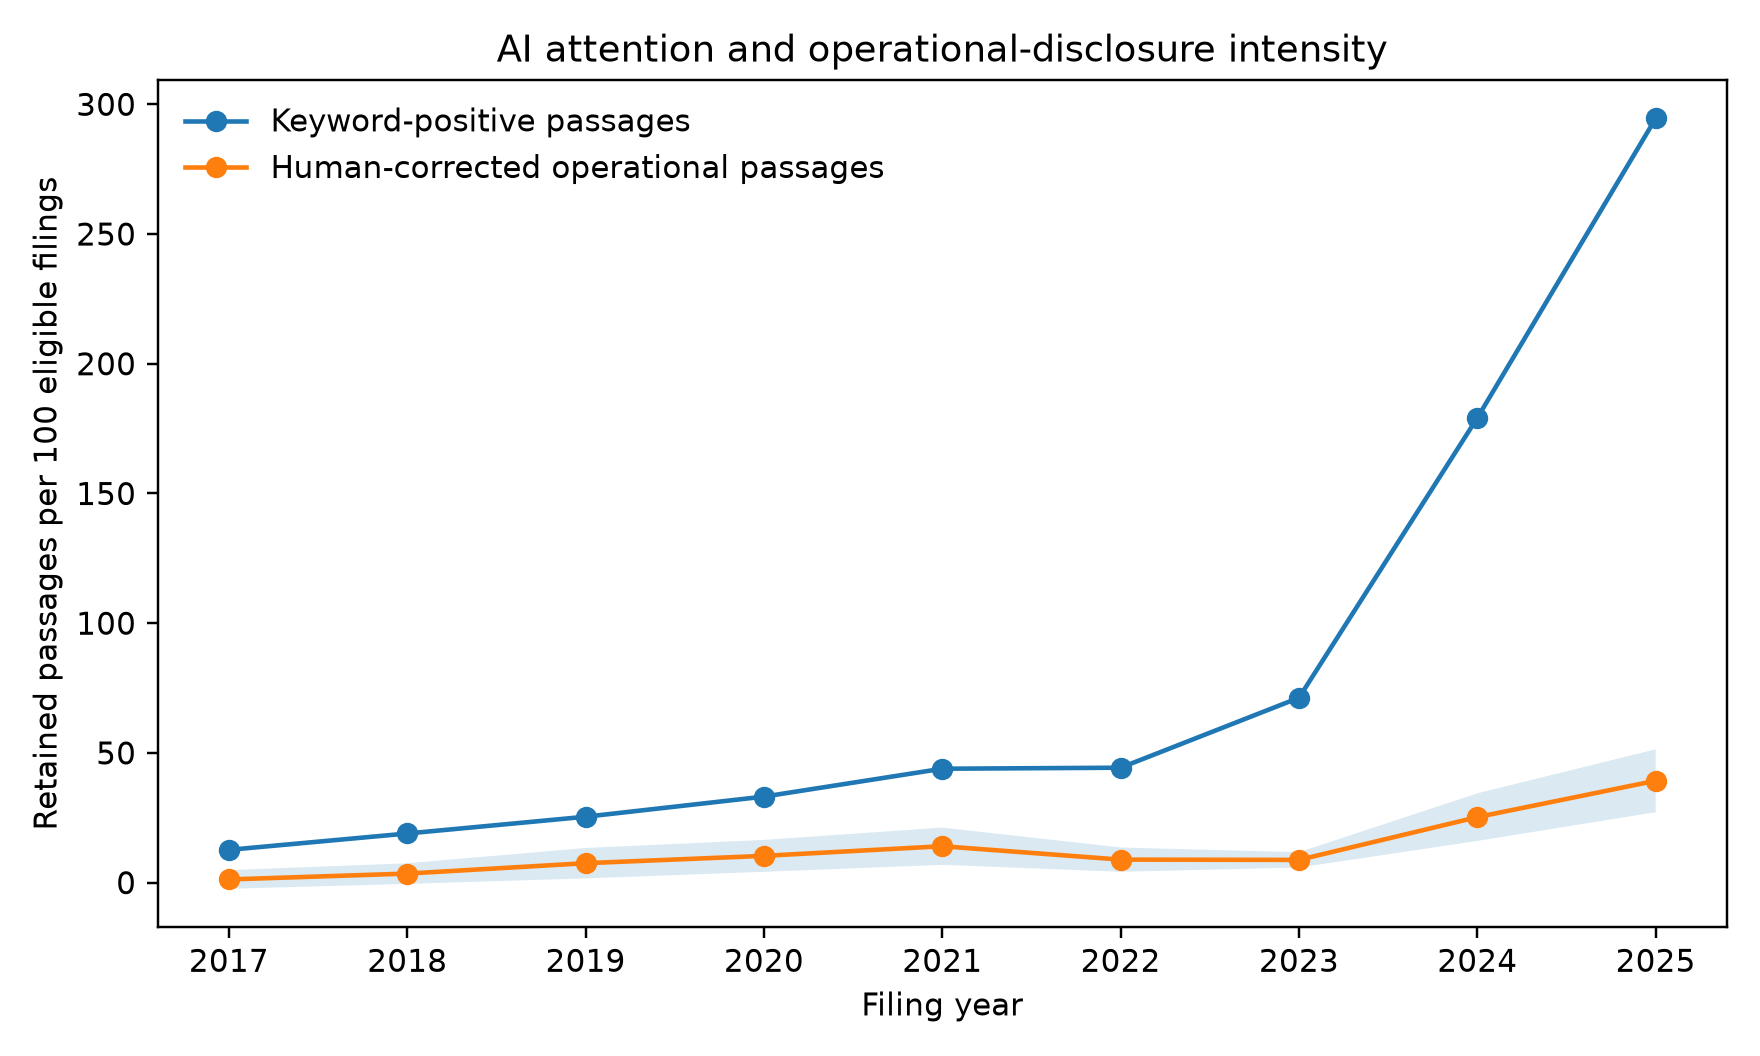
\includegraphics[width=0.92\textwidth]{reviewer_final/keyword_operational_benchmark.png}
\caption{AI attention and human-corrected operational-disclosure intensity}
\label{fig:attention_operational}
\par\smallskip\footnotesize
\textit{Note:} Values are retained candidate-passage windows per 100 processed
eligible filings. They are not lexical occurrence counts or firm adoption
rates. The shaded band is the approximate design-based interval for corrected
operational intensity.
\end{figure}

\end{document}
